\section*{ÔN TẬP KIỂM TRA CUỐI KÌ 1 - ĐỀ 05}
\setcounter{ex}{0}\setcounter{bt}{0}
\Opensolutionfile{ans}[ans/ansBTTeX5]

\begin{ex}%[VanLo HoaTrung, du an tex hoa tai lieu 10]%[0D4Y4-1]
Cặp số $(2 ;3)$ là nghiệm của bất phương trình nào sau đây?
\choice
{$2x-3y-1>0$}
{$x+y<0$}
{$4x>3y$}
{\True $x-3y+7 \le 0$}
\loigiai{
Thay tọa độ điểm $(2 ;3)$ lần lượt vào các bất phương trình ta thấy
\begin{itemize}
\item $2x-3y-1>0\colon2.2-3.3-1>0$ (sai);
\item $x+y<0\colon 2+3<0$ (sai);
\item $4x>3y\colon4.2>3.3$ (sai);
\item $x-3y+7 \le 0\colon2-3.3+7 \le 0$ (đúng).
\end{itemize}
}
\end{ex}

\begin{ex}%[0D2Y3-3]
Đồ thị dưới đây là của hàm số nào sau đây?
\begin{center}
\begin{tikzpicture}[scale=1, font=\footnotesize, line join=round, line cap=round,>=stealth]
\def\a{1} \def\b{-2} \def\c{-1} % Hệ số
\def\xmin{-1.5} \def\xmax{3.5}
\def\ymin{-2.5} \def\ymax{2}
\draw[->] (\xmin,0)--(\xmax,0) node [below]{$x$};
\draw[->] (0,\ymin)--(0,\ymax) node [left]{$y$};
\node at (0,0) [above right]{$O$};
\clip (\xmin+0.1,\ymin+0.1) rectangle (\xmax-0.1,\ymax-0.1);
\draw[smooth,samples=300] plot(\x,{\a*(\x)^2+\b*(\x)+\c});
\draw[dashed] (1,0)node[above]{$1$}--(1,-2)--(0,-2)node[left]{$-2$}
(0,-1)node[left]{$-1$} (2,0)node[above]{$2$};
\end{tikzpicture}
\end{center}
\choice
{$y=-x^2-2x+3$}
{$y=x^2+2x-2$}
{$y=2 x^2-4x-2$}
{\True $y=x^2-2x-1$}
\loigiai{
Đồ thị hàm số đi qua điểm $(0;1)\Rightarrow c=1$.\\
Vậy hàm số có đồ thị như hình vẽ là $y=x^2-2x-1$.
}
\end{ex}

\begin{ex}%[0H1Y1-3]
Phát biểu nào sau đây đúng?
\choice
{Hai vectơ không bằng nhau thì độ dài của chúng không bằng nhau}
{Hai vectơ không bằng nhau thì độ dài của chúng không cùng phương}
{\True Hai vectơ bằng nhau thì có giá trùng nhau hoặc song song nhau}
{Hai vectơ có độ dài không bằng nhau thì không cùng hướng}
\loigiai{
Hai vectơ bằng nhau thì cùng phương nên chúng có giá trùng nhau hoặc song song nhau.
}
\end{ex}

\begin{ex}%[0D2Y3-1]
Parabol $y=x^2+5x+6$ có tọa độ đỉnh là
\choice
{$\left(5;\dfrac{1}{2}\right)$}
{$\left(-\dfrac{5}{2};\dfrac{1}{2}\right)$}
{$\left(\dfrac{5}{2};\dfrac{1}{4}\right)$}
{\True $\left(-\dfrac{5}{2};-\dfrac{1}{4}\right)$}
\loigiai{
Tọa độ đỉnh của parabol là: $\heva{&x=-\dfrac{b}{2a}=-\dfrac{5}{2} \\& y=-\dfrac{\Delta}{4a}=-\dfrac{1}{4}}\Rightarrow I\left(-\dfrac{5}{2};-\dfrac{1}{4}\right)$.}
\end{ex}

\begin{ex}%[Trần Quốc, BG10-2022, Nhóm 9]%[0H1Y3-1]
Cho hai vectơ  $\vec{a}$, $\vec{b}$ bất kì và số thực $k$. Ta có $k\left(\vec{a}+\vec{b}\right)$ bằng
\choice
{$\vec{a}+k \vec{b}$}
{\True $k \vec{a}+k \vec{b}$}
{$k \vec{a}-k \vec{b}$}
{$k \vec{a}+\vec{b}$}
\loigiai{
Theo tính chất, ta có $k(\vec{a}+\vec{b})=k \vec{a}+k \vec{b}$.
}
\end{ex}

\begin{ex}%[Trần Minh,Chuyển sách Tex - 10, 11 (dự án 3)]%[0H2Y3-1]
Tam giác $ ABC$ có $ AB=9$ cm, $ AC=12$ cm và $ BC=15$ cm. Tính độ dài đường trung tuyến $ AM$ của tam giác đã cho.
\choice
{\True $ AM=\dfrac{15}{2}$ cm}
{$ AM=10$ cm}
{$ AM=9$ cm}
{$ AM=\dfrac{13}{2}$ cm}
\loigiai{
\immini{
Áp dụng hệ thức đường trung tuyến. Ta có
\begin{align*}
m_a^2&=\dfrac{b^2+c^2}{2}-\dfrac{a^2}{4}\\
&=\dfrac{12^2+9^2}{2}-\dfrac{15^2}{4}\\
&=\dfrac{225}{4}.\\
\Rightarrow m_a&=\dfrac{15}{2}.
\end{align*}

}
{
\begin{tikzpicture}[scale=1,font=\footnotesize,line join=round, line cap=round,>=stealth]
\tkzDefPoints{0/0/B,1/3/A,6/0/C}
\tkzDefMidPoint(C,B) \tkzGetPoint{M}
\tkzDrawPoints[fill=black](A,B,C,M)
\tkzDrawPolygon(A,B,C)
\tkzDrawSegments(A,M)
\tkzLabelPoints[above](A)
\tkzLabelPoints[below](B,C,M)
\end{tikzpicture}}
}
\end{ex}

\begin{ex}%[Phan Quốc Trí, Bai Giảng T10(2022)]%[0D1Y2-2]
Khẳng định nào sau đây là đúng?
\choice
{$ \mathbb{R}\subset\mathbb{Q} $}
{$ \mathbb{Z}\subset\mathbb{N} $}
{$ \mathbb{Q}\subset\mathbb{Z} $}
{\True $ \mathbb{N}\subset\mathbb{R} $}
\loigiai{
Ta có $ \mathbb{N}\subset\mathbb{Z}\subset\mathbb{Q}\subset\mathbb{R} $.
}
\end{ex}

\begin{ex}%[Đoàn Minh Tân]%[0D4Y5-1]
Tam thức $f(x)=x^2-12x-13$ nhận giá trị âm khi và chỉ khi
\choice
{$x<-13$ hoặc $x>1$}
{$x<-1$ hoặc $x>13$}
{$-13<x<1$}
{\True $-1<x<13$}
\loigiai{
Tam thức $f(x)=x^2-12x-13$ có $\Delta =196>0$, hai nghiệm $x_1=-1$, $x_2=13$ và hệ số $a=1>0$.\\
Bảng xét dấu của $f(x)$ như sau
\begin{center}

\begin{tikzpicture}
\tkzTabInit[nocadre=false, lgt=1.5, espcl=1.5]
{$x$ /0.6,$f(x)$ /0.6}
{$-\infty$,$-1$,$13$, $+\infty$}
\tkzTabLine{,+,0,-,0,+}
\end{tikzpicture}
\end{center}
Do đó $f(x)<0$ khi $-1<x<13$.
}
\end{ex}

\begin{ex}%[Phạm Ánh Thư, sách giảng dạy Toán 10]%[0D4Y4-4]
Cho hệ bất phương trình $\heva{& x+3y-2\geq 0\\ & 2x+y+1\leq 0}$. Trong các điểm sau, điểm nào thuộc miền nghiệm của hệ bất phương trình?
\choice
{$M\left(0;1\right)$}
{\True $N\left(-1;1\right)$}
{$P\left(1;3\right)$}
{$Q\left(-1;0\right)$}
\loigiai{
Thay toạ độ điểm $N\left(-1;1\right)$ vào hệ bất phương trình ta có $\heva{& -1+3-2\geq 0\\ & -2+1+1\leq 0}$ (đúng). Do đó, điểm $N$ thuộc miền nghiệm của hệ bất phương trình.
}

\end{ex}

\begin{ex}%[Lương Như Quỳnh, TLDH5]%[0D1Y1-3]
Cho mệnh đề \lq\lq $\forall x\in \mathbb{R},\,x^2-x+7<0$\rq\rq. Hỏi mệnh đề nào là mệnh đề phủ định của mệnh đề trên?
\choice
{\True $\exists x\in \mathbb{R},\,x^2-x+7\ge 0$}
{$\forall x\in \mathbb{R},\,x^2-x+7 > 0$}
{$\forall x\in \mathbb{R},\,x^2-x+7 < 0$}
{$\nexists x\in \mathbb{R},\,x^2-x+7 < 0$}
\loigiai{
Ta có phủ định của mệnh đề \lq\lq$\forall x\in X,P(x)$\rq\rq\,\, là mệnh đề \,\lq\lq$\exists x\in X,\overline{P(x)}$\rq\rq.\\
Suy ra mệnh đề phủ định của mệnh đề đã cho là \lq\lq $\exists x\in \mathbb{R},\,x^2-x+7\geq 0$\rq\rq\,.
}
\end{ex}

\begin{ex}%[Trần Minh,Chuyển sách Tex - 10, 11 (dự án 3)]%[0H2Y3-1]
Tam giác $ ABC$ có $ AB=\sqrt{2}$, $AC=\sqrt{3}$ và $ \widehat{C}=45^\circ $. Tính độ dài cạnh $ BC$.
\choice
{$ BC=\sqrt{5}$}
{\True $ BC=\dfrac{\sqrt{6}+\sqrt{2}}{2}$}
{$ BC=\dfrac{\sqrt{6}-\sqrt{2}}{2}$}
{$ BC=\sqrt{6}$}
\loigiai
{Theo định lí hàm cô-sin, ta có\\
$ AB^2=AC^2+BC^2-2\cdot AC\cdot BC\cdot \cos \widehat{C}\Rightarrow {(\sqrt{2} )}^2={(\sqrt{3} )}^2+BC^2-2\cdot \sqrt{3}\cdot BC\cdot \cos 45^\circ $ \\
$ \Rightarrow BC=\dfrac{\sqrt{6}+\sqrt{2}}{2}$.}
\end{ex}

\begin{ex}%[0H2Y2-1]
Cho $\overrightarrow{a} $ và $\overrightarrow{b} $ là hai véc-tơ cùng hướng và đều khác $\overrightarrow{0} $. Mệnh đề nào sau đây đúng?
\choice
{\True $\overrightarrow{a} \cdot \overrightarrow{b}=\big| \overrightarrow{a}\big| \cdot \big| \overrightarrow{b}\big| $}
{$\overrightarrow{a} \cdot \overrightarrow{b}=0$}
{$\overrightarrow{a} \cdot \overrightarrow{b}=-1$}
{$\overrightarrow{a} \cdot \overrightarrow{b}=-\big| \overrightarrow{a}\big| \cdot \big| \overrightarrow{b}\big| $}
\loigiai{
Ta có $\overrightarrow{a} \cdot \overrightarrow{b}=\big| \overrightarrow{a}\big| \cdot \big| \overrightarrow{b}\big| \cdot \cos\left(\overrightarrow{a},\overrightarrow{b}\right)$. \\
Do $\overrightarrow{a} $ và $\overrightarrow{b} $ là hai véc-tơ cùng hướng nên $ \left(\overrightarrow{a},\overrightarrow{b}\right)=0^\circ $. \\
Vậy $\overrightarrow{a} \cdot \overrightarrow{b}=\big| \overrightarrow{a}\big| \cdot \big| \overrightarrow{b}\big| $.
}
\end{ex}

\begin{ex}%[0D4Y5-1]
Tìm $m$ để biểu thức $f(x)=(m-3) x^2+(2-m) x+1$ là tam thức bậc hai.
\choice
{$m=3$}
{\True $m \neq 3$}
{$m<3$}
{$m>3$}
\loigiai{
$f(x)=(m-3) x^2+(2-m) x+1$ là tam thức bậc hai khi $m-3\neq 0 $ hay $m\neq 3$.
}
\end{ex}


\begin{ex}%[0D4B5-2]
Cho các mệnh đề\\
(I) Với mọi $x \in [-1;4]$ thì $-x^2+4x+5 \geq 0$.\\
(II) Với mọi $x \in (-\infty;4) \cup (5;10)$ thì $x^2+9x-10>0$. \\
(III) Với mọi $x \in [2;3]$ thì $x^2-5x+6 \leq 0$.
\choice
{\True Mệnh đề (I) và (III) đúng}
{Chỉ mệnh đề (I) đúng}
{Chỉ mệnh đề (III) đúng}
{Cả ba mệnh đề đều sai}
\loigiai{
\begin{itemize}
\item $-x^2+4x+5 \geq 0 \Leftrightarrow -1 \leq x \leq 5$, suy ra mệnh đề (I) đúng.
\item $x^2+9x-10>0 \Leftrightarrow \hoac{& x>1 \\& x<-10}$, suy ra mệnh đề (II) sai.
\item $x^2-5x+6 \leq 0 \Leftrightarrow 2 \leq x \leq 3$, suy ra mệnh đề (III) đúng.
\end{itemize}
}
\end{ex}

\begin{ex}%[Lê Hồng Phi, Dự án TLDH5-Nhóm Latex, 2020]%[0D1B1-4]
Mệnh đề nào sau đây {\bf sai}?
\choice
{Nếu $\triangle ABC$ có hai góc cùng bằng $60^\circ$ thì nó là tam giác đều}
{\True Hai tam giác có diện tích bằng nhau khi và chỉ khi hai tam giác đó bằng nhau}
{Nếu $n$  là số nguyên lẻ thì $3n+1$  là số nguyên chẵn}
{Nếu hai số $a$ và $b$ cùng chia hết cho $c$ thì $a+b$ chia hết cho $c$}
\loigiai
{\immini{Hai tam giác $ABC$ và $DBC$ có diện tích bằng nhau nhưng chúng không bằng nhau.}{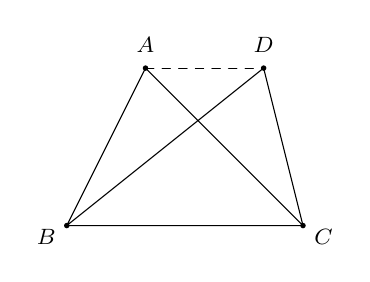
\begin{tikzpicture}[scale=1, font=\footnotesize, line join=round, line cap=round,>=stealth]
\path (0,0)coordinate (B) (3,0) coordinate (C) (1,2) coordinate (A) (2.5,2) coordinate (D);
\draw (A)--(B)--(C)--cycle (B)--(D)--(C);
\draw[dashed] (A)--(D);
\foreach \p/\g in {B/-150,C/-30,A/90,D/90} \fill[black] (\p) circle(1pt)+(\g:0.3) node{$\p$};
\end{tikzpicture}}
}
\end{ex}

\begin{ex}%[Võ Thị Thùy Trang, Dự án TLDH5]%[0D2B1-1]
Cho hàm số $y=\heva{&\dfrac{3-x}{x-1}\ \text{khi}  \ x < 0\\& {x^2}-2x+2\ \text{khi}\ x\ge 0}
$. Tính $f\left(2\right)$, ta được kết quả
\choice
{$1$}
{\True $2$}
{$-1$}
{$-2$}
\loigiai{
Ta có $f(2)=2^2-4+2=2$.}
\end{ex}

\begin{ex}%[Trần Minh,Chuyển sách Tex - 10, 11 (dự án 3)]%[0H1B3-2]
Cho tam giác $ABC$ và một điểm $M$ tùy ý. Mệnh đề nào sau đây đúng?
\choice
{$2\overrightarrow{MA}+\overrightarrow{MB}-3\overrightarrow{MC}=\overrightarrow{AC}+2\overrightarrow{BC}$}
{$2\overrightarrow{MA}+\overrightarrow{MB}-3\overrightarrow{MC}=2\overrightarrow{AC}+\overrightarrow{BC}$}
{\True $2\overrightarrow{MA}+\overrightarrow{MB}-3\overrightarrow{MC}=2\overrightarrow{CA}+\overrightarrow{CB}$}
{$2\overrightarrow{MA}+\overrightarrow{MB}-3\overrightarrow{MC}=2\overrightarrow{CB}-\overrightarrow{CA}$}
\loigiai{
Ta có $2\overrightarrow{MA}+\overrightarrow{MB}-3\overrightarrow{MC}=2\overrightarrow{MC}+2\overrightarrow{CA}+\overrightarrow{MC}+\overrightarrow{CB}-3\overrightarrow{MC}=2\overrightarrow{CA}+\overrightarrow{CB}$.
}
\end{ex}

\begin{ex}%[Lê Minh Thiện Anh, Dự án BG10-Lần2]%[0H1B1-1]
Cho tam giác $MNP$, có thể xác định được tối đa bao nhiêu véc-tơ khác $\overrightarrow{0}$ có điểm đầu và điểm cuối là các đỉnh $M$, $N$, $P$?
\choice
{$3$}
{$27$}
{\True $6$}
{$9$}
\loigiai{
Với hai điểm phân biệt $A$ và $B$ ta sẽ có hai vectơ khác $\overrightarrow{0}$ đó là $\overrightarrow{AB}$ và $\overrightarrow{BA}$.\\
Vậy với $3$ điểm $M$, $N$, $P$ có tất cả $6$ véc-tơ thỏa mãn.
}
\end{ex}

\begin{ex}%[Word: Nguyễn Văn Mến, LaTeX: Nguyễn Tài Tuệ, PB: Nguyễn Tấn Linh]%[0D4B4-1]
\immini[thm]{ Phần gạch chéo trong hình vẽ dưới đây (không bao gồm đường thẳng d) là miền nghiệm cuả bất phương trình bậc nhất hai ẩn nào sau đây?
\choice
{$2x-y<0$}
{$x-2y<2$}
{\True $2y-x<-2$}
{$2x-y>1$}}{\begin{tikzpicture}[line join=round, line cap=round,>=stealth]
\tikzset{label style/.style={font=\footnotesize}}
\begin{scope}
\clip (-2.5,-3) rectangle (3,2);
\fill[pattern=north east lines] (-4.5,-3.25)--(7,-3.25)--(7,2.5)--cycle;
\draw (6,2)--(-4,-3) node [pos=0.45, above, sloped] {};
\end{scope}
\draw[->] (-2.5,0)--(3,0) node[below]{$x$};
\draw[->] (0,-3)--(0,2) node[left]{$y$};
\draw (0,0) node[below left]{$O$};
\foreach \x in {2}
\draw[thin] (\x,1pt)--(\x,-1pt) node [below] {$\x$};
\foreach \y in {-1}
\draw[thin] (1pt,\y)--(-1pt,\y) node [left] {$\y$};
\end{tikzpicture}}
\loigiai{
%Fb tác giả: Nguyễn Văn Mến\\
Đường thẳng d đi qua hai điểm $A(0;-1)$ và $B(2;0)$ nên có phương trình là $y=\dfrac{1}{2}x-1$.\\
Lại có điểm $O(0;0)$ không thuộc vào miền nghiệm nên $y<\dfrac{1}{2}x-1$ (vì $0<\dfrac{1}{2} \cdot 0-1$ \textbf{không đúng}).\\
Hay $2y<x-2 \Leftrightarrow 2y-x<-2$.}
\end{ex}

\begin{ex}%[Trần Minh,Chuyển sách Tex - 10, 11 (dự án 3)]%[0H1B2-4]
\immini
{
Cho hình bình hành $ABCD$ có $O$ là giao điểm của hai đường chéo. Gọi $E$, $ F$ lần lượt là trung điểm của $AB$, $ BC$. Đẳng thức nào sau đây \textbf{sai}?
\choice
{$\overrightarrow{DO}=\overrightarrow{EB}-\overrightarrow{EO}$}
{$\overrightarrow{OC}=\overrightarrow{EB}+\overrightarrow{EO}$}
{$\overrightarrow{OA}+\overrightarrow{OC}+\overrightarrow{OD}+\overrightarrow{OE}+\overrightarrow{OF}=\overrightarrow{0}$}
{\True $\overrightarrow{BE}+\overrightarrow{BF}-\overrightarrow{DO}=\overrightarrow{0}$}
}
{
\begin{tikzpicture}[scale=0.9, font=\footnotesize, line join = round, line cap = round,>=stealth]
\tkzDefPoints{0/0/A,2/2/B,4/0/D}
\coordinate (C) at ($(B)+(D)-(A)$);
\tkzDefMidPoint(A,C) \tkzGetPoint{O}
\tkzDefMidPoint(A,B) \tkzGetPoint{E}
\tkzDefMidPoint(C,B) \tkzGetPoint{F}
\tkzDrawPoints[fill=black](A,B,C,D,O,E,F)
\tkzDrawPolygon(A,B,D,C)
\tkzDrawSegments(C,B A,D O,E O,F)
\tkzLabelPoints[above](B,C,F)
\tkzLabelPoints[below](A,D,O)
\tkzLabelPoints[left](E)
\end{tikzpicture}
}
\loigiai{
Ta có $OF$, $ OE$ lần lượt là đường trung bình của tam giác $\Delta BCD$ và $\Delta ABC$. \\
$\Rightarrow BEOF$ là hình bình hành.\\
$\Rightarrow \overrightarrow{BE}+\overrightarrow{BF}=\overrightarrow{BO}.\\
\Rightarrow \overrightarrow{BE}+\overrightarrow{BF}-\overrightarrow{DO}=\overrightarrow{BO}-\overrightarrow{DO}=\overrightarrow{OD}-\overrightarrow{OB}=\overrightarrow{BD}$.
}
\end{ex}

\begin{ex}%[0D3B2-4]
Tổng bình phương các nghiệm của	 phương trình $3\sqrt{x-1}=\sqrt{x^2+8x-11}$ là
\choice
{\True 4}
{8}
{5}
{7}
\loigiai{\begin{eqnarray*} 3\sqrt{x-1}=\sqrt{x^2+8x-11}
&\Rightarrow& 9\left(x-1\right) = x^2+8x-11\\
& \Rightarrow& x^2 -x-2= 0\\
& \Rightarrow & \hoac{& x=2  \\& x=-1.}
\end{eqnarray*}
Chỉ có nghiệm $x=2$ thỏa mãn phương trình ban đầu.\\
Nên phương trình có tập nghiệm $S = \left\{ 2 \right\}$. \\
Vậy tổng bình phương các nghiệm là $4$.}
\end{ex}

\begin{ex}%[0D3B2-4]
Số nghiệm của phương trình $\sqrt{2x^2-8x-5}=5-3x$ là
\choice
{$2$}
{\True $0$}
{$1$}
{vô số}
\loigiai{
Trước hết ta giải bất phương trình $5-3x\geq 0\Leftrightarrow x\leq \dfrac{5}{3}.\; (*)$
\allowdisplaybreaks
\begin{eqnarray*}
&&\sqrt{2x^2-8x-5}=5-3x\\
&\Rightarrow&2x^2-8x-5=(5-3x)^2\\
&\Rightarrow&7x^2-22x+30=0. \; \text{ phương trình này vô nghiệm.}
\end{eqnarray*}
Vậy phương trình đã cho vô nghiệm.
}
\end{ex}

\begin{ex}%[0D3B2-4]
Tổng các nghiệm của phương trình $\sqrt{3x^2+23x+29}=x+4$ là
\choice
{\True $-1$}
{$-\dfrac{15}{2}$}
{$-\dfrac{13}{2}$}
{$0$}
\loigiai{
Trước hết ta giải bất phương trình $x+4\geq 0\Leftrightarrow x\geq -4.\; (*)$
\allowdisplaybreaks
\begin{eqnarray*}
&&\sqrt{3x^2+23x+29}=x+4\\
&\Rightarrow&3x^2+23x+29=(x+4)^2\\
&\Rightarrow&2x^2+15x+13=0\\
&\Rightarrow&\hoac{&x=-1\\&x=-\dfrac{13}{2}.}
\end{eqnarray*}
Trong hai giá trị trên, chỉ có $x=-1$ thỏa mãn $(*)$.\\
Vậy phương trình đã cho có tập nghiệm $S=\left\{-1\right\}$, nên tổng của chúng bằng $-1$.
}
\end{ex}

\begin{ex}%[0D2B3-1]
Đường thẳng nào sau đây là trục đối xứng của đồ thị hàm số $y=2x^2+8x+5$?
\choice
{\True$x=-2$}
{$x=2$}
{$x=4$}
{$x=-4$}
\loigiai{
Trục đối xứng của đồ thị hàm số $y=2x^2+8x+5$ là đường thẳng $x=\dfrac{-b}{2a}=\dfrac{-8}{2\cdot2}=-2$.
}
\end{ex}

\begin{ex}%[0H2B1-2]
Tính giá trị biểu thức $P=\cos 30^\circ\cos 60^\circ-\sin 30^\circ\sin 60^\circ$.
\choice
{$P=\sqrt{3}$}
{$P=\dfrac{\sqrt{3}}{2}$}
{$P=1$}
{\True $P=0$}
\loigiai
{Vì $30^\circ$ và $60^\circ$ là hai góc phụ nhau nên $\heva{& \sin 30^\circ=\cos 60^\circ \\
& \sin 60^\circ=\cos 30^\circ \\
}$.\\
$\Rightarrow P=\cos 30^\circ\cos 60^\circ-\sin 30^\circ\sin 60^\circ=\cos 30^\circ\cos 60^\circ-\cos 60^\circ\cos 30^\circ=0$.}
\end{ex}

\begin{ex}%[0D4B4-4]
Cặp số $(x;y)$ nào sau đây là một nghiệm của hệ bất phương trình $\heva{&2x+3y-1>0\\&5x-y+4\leq0}$?
\choice
{\True $(0;4)$}
{$(0;0)$}
{$(-2;-4)$}
{$(-3;-4)$}
\loigiai{Thay cặp số $(0;4)$ vào hệ bất phương trình đã cho, ta có
$\heva{&2 \cdot 0 + 3 \cdot 4-1=11>0\\&5 \cdot 0-4+4 = 0 \leq 0}$
(đúng).
}
\end{ex}

\begin{ex}%[Phan Anh]%[0D2B1-2]
Tìm tập xác định $\mathscr{D}$ của hàm số $y=\dfrac{x+1}{(x-3)\sqrt{2x-1}}$.
\choice
{$\mathscr{D}=\mathbb{R}$}
{$\mathscr{D}=\left(-\dfrac{1}{2};+\infty \right)\setminus\left\{3\right\}$}
{$\mathscr{D}=\left[\dfrac{1}{2};+\infty \right)\setminus\left\{3\right\}$}
{\True $\mathscr{D}=\left(\dfrac{1}{2};+\infty \right)\setminus\left\{3\right\}$}
\loigiai{
Hàm số xác định khi $\heva{
& x-3\ne 0 \\
& 2x-1>0}\Leftrightarrow \heva{
& x\ne 3 \\
& x>\dfrac{1}{2}.}$\\
Vậy tập xác định của hàm số là $\mathscr{D}=\left(\dfrac{1}{2};+\infty \right)\setminus\left\{3\right\}$.}
\end{ex}

\begin{ex}%[Phan Quốc Trí, Bai Giảng T10(2022)]%[0D1B3-2]
Cho tập hợp $ A=[-2;3] $ và $ B=(1;5] $. Khi đó $ A\setminus B $ là
\choice
{$(-2;1]$}
{$(-2;-1)$}
{$[-2;1) $}
{\True $[-2;1]$}
\loigiai{
Ta có $ A\setminus B =[-2;3]\setminus(1;5]= [-2;1]$.
}
\end{ex}

\begin{ex}%[Lê Minh Thiện Anh, Dự án BG10-Lần2]%[0H1B1-1]
Cho tam giác $MNP$, có thể xác định được tối đa bao nhiêu véc-tơ khác $\overrightarrow{0}$ có điểm đầu và điểm cuối là các đỉnh $M$, $N$, $P$?
\choice
{$3$}
{$27$}
{\True $6$}
{$9$}
\loigiai{
Với hai điểm phân biệt $A$ và $B$ ta sẽ có hai vectơ khác $\overrightarrow{0}$ đó là $\overrightarrow{AB}$ và $\overrightarrow{BA}$.\\
Vậy với $3$ điểm $M$, $N$, $P$ có tất cả $6$ véc-tơ thỏa mãn.
}
\end{ex}

\begin{ex}%[Trần Minh,Chuyển sách Tex - 10, 11 (dự án 3)]%[0H1B3-1]
Cho tam giác $ABC$ vuông tại $A$, $M$ là trung điểm của $BC$. Khẳng định nào sau đây đúng?
\choice
{$\overrightarrow{AM}=\overrightarrow{MB}=\overrightarrow{MC}$}
{$\overrightarrow{MB}=\overrightarrow{MC}$}
{\True $\overrightarrow{MB}=-\overrightarrow{MC}$}
{$\overrightarrow{AM}=\dfrac{\overrightarrow{BC}}{2}$}
\loigiai{
Vì $M$ là trung điểm của $BC$ nên $\overrightarrow{MB}+\overrightarrow{MC}=\overrightarrow{0}\Leftrightarrow \overrightarrow{MB}=-\overrightarrow{MC}$. }
\end{ex}

\begin{ex}%[0H2B1-1]
Cho $\alpha $ là góc tù. Khẳng định nào sau đây là \textbf{đúng}?
\choice
{$\sin \alpha <0$}
{$\cos \alpha >0$}
{\True $\tan \alpha <0$}
{$\cot \alpha >0$}
\loigiai{}
\end{ex}

\begin{ex}%[0H2B2-1]
Cho tam giác $ABC$ đều có cạnh bằng $a$. Tích vô hướng $\overrightarrow{AB}\cdot\overrightarrow{AC}$ bằng
\choice
{$2a^2$}
{$-\dfrac{a^2\sqrt{3}}{2}$}
{$-\dfrac{a^2}{2}$}
{\True $\dfrac{a^2}{2}$}
\loigiai{
\immini{
Ta có $\overrightarrow{AB}\cdot\overrightarrow{AC}=AB\cdot AC\cdot\cos 60^\circ=a\cdot a\cdot\dfrac{1}{2}=\dfrac{a^2}{2}$.
}{
\begin{tikzpicture}[scale=1, font=\footnotesize, line join=round, line cap=round, >=stealth]
\tkzDefPoints{0/0/B,3/0/C}
\tkzDefPointsBy[rotation=center B angle 60](C){A}
\draw (B)--(C);
\draw[->] (A)--(B);
\draw[->] (A)--(C);
\tkzLabelPoints[above](A)
\tkzLabelPoints[below left](B)
\tkzLabelPoints[below right](C)
\tkzMarkAngle[size=0.5,mark=](B,A,C)
\end{tikzpicture}
}
}
\end{ex}

\begin{ex}%[0H2B2-1]
Cho hình chữ nhật $ABCD$ có $AB=a$ và $AD=a\sqrt{2}$. Gọi $K$ là trung điểm của cạnh $AD$. Tính $\overrightarrow{BK}\cdot\overrightarrow{AC}$.
\choice
{\True $\overrightarrow{BK}\cdot\overrightarrow{AC}=0$}
{$\overrightarrow{BK}\cdot\overrightarrow{AC}=-a^2\sqrt{2}$}
{$\overrightarrow{BK}\cdot\overrightarrow{AC}=a^2\sqrt{2}$}
{$\overrightarrow{BK}\cdot\overrightarrow{AC}=2a^2$}
\loigiai
{	\immini{Ta có $AC=BD=\sqrt{AB^2+AD^2}=\sqrt{2a^2+a^2}=a\sqrt{3}$.\\
Ta có $\heva{& \overrightarrow{BK}=\overrightarrow{BA}+\overrightarrow{AK}=\overrightarrow{BA}+\dfrac{1}{2}\overrightarrow{AD} \\
& \overrightarrow{AC}=\overrightarrow{AB}+\overrightarrow{AD} \\
}$}{\begin{tikzpicture}[scale=0.7]
\tkzDefPoints{0/0/B,5/0/C,0/2/A}
\coordinate (D) at ($(A)+(C)-(B)$);
\coordinate (K) at ($(A)!0.5!(D)$);
\tkzDrawSegments(A,B B,C C,D D,A A,C B,K)
\tkzDrawPoints[fill=black](A,B,C,D,K)
\tkzLabelPoints[above](A,K,D)\tkzLabelPoints[below](B,C)
\end{tikzpicture}}
\noindent \begin{eqnarray*}
\Rightarrow\overrightarrow{BK}\cdot\overrightarrow{AC}&=&\left(\overrightarrow{BA}+\dfrac{1}{2}\overrightarrow{AD} \right)(\overrightarrow{AB}+\overrightarrow{AD} )\\
&=&\overrightarrow{BA}\cdot\overrightarrow{AB}+\overrightarrow{BA}\cdot\overrightarrow{AD}+\dfrac{1}{2}\overrightarrow{AD}\cdot\overrightarrow{AB}+\dfrac{1}{2}\overrightarrow{AD}\cdot\overrightarrow{AD}=-a^2+0+0+\dfrac{1}{2}{{(a\sqrt{2} )}^2}=0.
\end{eqnarray*}}
\end{ex}

\begin{ex}%[0D2B1-3]
Xét sự biến thiên của hàm số $ y=\dfrac{1}{x^2}$. Mệnh đề nào sau đây \textbf{đúng}?
\choice
{\True Hàm số đồng biến trên $(-\infty ;0)$, nghịch biến trên $(0;+\infty)$}
{Hàm số đồng biến trên $(0;+\infty)$, nghịch biến trên $(-\infty ;0)$}
{Hàm số đồng biến trên $(-\infty ;1)$, nghịch biến trên $(1;+\infty)$}
{Hàm số nghịch biến trên $(-\infty ;0)\cup(0;+\infty)$}
\loigiai{
TXĐ: $\mathscr{D}= \mathbb{R} \setminus \{0\}$.
\begin{itemize}
\item Lấy $x_1, x_2 \in (0; +\infty): 0< x_1 < x_2$. Khi đó $x_2-x_1>0$ và $x_1+x_2>0$.\\
Xét hiệu: $f(x_1) -f(x_2)= \dfrac{1}{x_1^2} - \dfrac{1}{x_2^2} = \dfrac{x_2^2-x_1^2}{x_1^2\cdot x_2^2}= \dfrac{(x_2-x_1)(x_2+x_1)}{x_1^2\cdot x_2^2} > 0$	$\Rightarrow f(x_1) > f(x_2)$.\\
Suy ra hàm số nghịch biến trên khoảng $(0;+\infty)$.
\item Lấy $x_1, x_2 \in (-\infty;0): x_1 < x_2<0$. Khi đó $x_2-x_1>0$ và $x_1+x_2<0$.\\
Xét hiệu: $f(x_1)-f(x_2)= \dfrac{1}{x_1^2} - \dfrac{1}{x_2^2} = \dfrac{x_2^2-x_1^2}{x_1^2\cdot x_2^2}= \dfrac{(x_2-x_1)(x_2+x_1)}{x_1^2\cdot x_2^2} < 0$	$\Rightarrow f(x_1) < f(x_2)$.\\
Suy ra hàm số đồng biến trên khoảng $(-\infty;0)$.
\end{itemize}
}
\end{ex}


\begin{ex}%[0D1K3-3]
Lớp 10A có $51$ bạn học sinh trong đó có $31$ bạn học tiếng Anh và $27$ bạn học tiếng Nhật. Lớp 10A có bao nhiêu bạn học cả tiếng Anh và tiếng Nhật?
\choice
{\True $7$}
{$9$}
{$5$}
{$12$}
\loigiai
{
\immini
{
Gọi $A$, $B$ lần lượt là tập hợp các học sinh học tiếng Anh và học tiếng Nhật.\\
Số học sinh học tiếng Anh: $n(A)=31$.\\
Số học sinh biết học tiếng Nhật: $n(B)=27$.
}
{
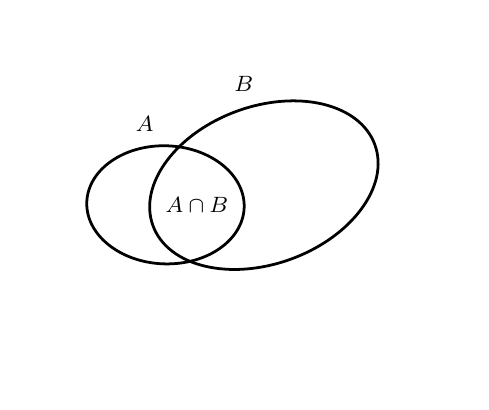
\begin{tikzpicture}[xscale=0.5,yscale=0.5, font=\footnotesize, line join=round, line cap=round, >=stealth]
\clip(1,-4) rectangle (12,5);
\draw [rotate around={-2:(4.5,0.5)},line width=1pt] (4.5,0.5) ellipse (2cm and 1.5cm);
\draw [rotate around={20:(7,1)},line width=1pt] (7,1) ellipse (3cm and 2cm);
\draw (6,4) node[anchor=north west] {$B$};
\draw (3.5,3) node[anchor=north west] {$A$};
\draw (5.3,.5) node{$A \cap B$};
\end{tikzpicture}
}
Suy ra số học sinh học cả tiếng Anh và Nhật là $n(A \cap B)= n(A)+n(B)-n(A\cup B)=31+27-51=7$.
}
\end{ex}
\Closesolutionfile{ans}
\begin{ex}[1,0 điểm]
Vẽ đồ thị hàm số $y=-2x^2+3x+5$.
\end{ex}

\begin{ex}[0,5 điểm]%[Hoàng Thanh Phương, BG10-2022-Đợt 2, Nhóm 3]%[0D4B5-1]
Giải bất phương trình sau $2x^2+3x-14>= 0$ bằng cách lập bảng xét dấu.
\loigiai{

}
\end{ex}

\begin{ex}[0,5 điểm]%[Phan Anh]%[Dự án giáo án 10]%[0H1B2-5]
Cho hình vuông $ABCD$ có cạnh bằng $1$. Tính độ dài của vectơ $\overrightarrow{u}=3\overrightarrow{AC}-7\overrightarrow{AB}$.
% \choice
% {\True $|\overrightarrow{u}|=5$}
% {$|\overrightarrow{u}|=12\sqrt{2}-7$}
% {$|\overrightarrow{u}|=17$}
% {$|\overrightarrow{u}|=13$}
\loigiai{
\immini{Ta có $\overrightarrow{u}=3\left(\overrightarrow{AB}+\overrightarrow{AD}\right)-7\overrightarrow{AB}=-4\overrightarrow{AB}+3\overrightarrow{AD}$.\\
Dựng $E$, $F$, $G$ sao cho $\overrightarrow{AE}=-4\overrightarrow{AB}$,  $\overrightarrow{AF}=3\overrightarrow{AD}$ và $AEGF$ là hình bình hành.\\
Vì $AB\perp AD$ nên $AE\perp AF$. Do đó $AEGF$ là hình chữ nhật.\\
Vậy $\overrightarrow{u}=\overrightarrow{AG}$ và
$\left|\overrightarrow{u}\right|=\left|\overrightarrow{AG}\right|=AG=EF=\sqrt{AE^2+AF^2}=\sqrt{4^2+3^2}=5$.}
{\begin{tikzpicture}[scale=1, font=\footnotesize, line join=round, line cap=round,>=stealth]
\path (0,0)coordinate (B)
(1,0) coordinate (C)
($(B)!1!90:(C)$) coordinate (A)
($(A)+(C)-(B)$) coordinate (D)
($(A)!-4!(B)$) coordinate (E)
($(A)!3!(D)$) coordinate (F)
($(E)+(F)-(A)$) coordinate (G);
\draw (A)--(B)--(C)--(D)--cycle;
\draw[->] (A)--(E);
\draw[->] (A)--(F);
\draw[->] (A)--(G);
\draw[dashed] (E)--(G)--(F);
\foreach \x/\pos in {A/180,B/-150,C/-30,D/60,E/150,F/0,G/30} \fill (\x) circle(1pt) node[{shift=(\pos:0.25)}]{$\x$};
\end{tikzpicture}}
}

\end{ex}

\begin{ex}[0,5 điểm]%[Nguyễn Tất Thu, BG10-2022]%[0H2K2-4]
Cho tam giác $ABC$. Tập hợp các điểm $M$ thỏa $\left( \overrightarrow{MA}+2\overrightarrow{MB} \right)\left( \overrightarrow{MB}+2\overrightarrow{MC} \right)=0$ là
% \choice
% {Đường thẳng vuông góc với $AB$}
% {Đoạn thẳng}
% {Đường thẳng song song với $AB$}
% {\True Đường tròn}
\loigiai{
Gọi $D$ và $E$ là các điểm thoả mãn: \[\overrightarrow{DA}+2\overrightarrow{DB}=\overrightarrow{0},\ \overrightarrow{EB}+2\overrightarrow{EC}=\overrightarrow{0}.\] Ta có
\[\left( \overrightarrow{MA}+2\overrightarrow{MB} \right)\left( \overrightarrow{MB}+2\overrightarrow{MC} \right)=0\Leftrightarrow \overrightarrow{MD}\cdot \overrightarrow{ME}=0.\]
Tập hợp điểm $M$ là đường tròn đường kính $DE$.
}
\end{ex}

\begin{ex}[0,5 điểm]%[Đề kiểm tra HK2 môn Toán 10 trường THPT Nguyễn Thượng Hiền]%[Đoàn Minh Tân, 10EX-HK2-2223]%[0D4T5-6]
      Hai chiếc máy bay đồng thời rời khỏi sân bay Đà Nẵng, một chiếc bay thẳng về phía Bắc và chiếc còn lại bay thẳng về phía Đông. Chiếc máy bay về phía Bắc nhanh hơn 50 dặm/giờ so với chiếc máy bay về hướng Đông. Sau 3 giờ, những chiếc máy bay cách nhau 2440 dặm. Tìm tốc độ của mỗi máy bay.
\end{ex}